
%----------------------------------------------------------------------------------------
%	PACKAGES AND OTHER DOCUMENT CONFIGURATIONS
%----------------------------------------------------------------------------------------

\documentclass[a4paper,12pt]{article}


%----------------------------------------------------------------------------------------
%	PACKAGES AND OTHER DOCUMENT CONFIGURATIONS
%----------------------------------------------------------------------------------------

\usepackage{amsmath,amsfonts,stmaryrd,amssymb} % Math packages

\usepackage{enumerate} % Custom item numbers for enumerations

\usepackage{mhchem}
\usepackage[hidelinks]{hyperref}
%\hypersetup{
%	colorlinks = true,
%	urlcolor=black,
%	filecolor=black,
%	citecolor=black,
%	linkcolor=black
%	}

\usepackage{multirow}
\usepackage{tabularx}
\usepackage{booktabs}
\usepackage{booktabs}
\usepackage{siunitx}
\usepackage{subfigure}
\usepackage{xcolor}

\usepackage[italian]{babel}

\usepackage[ruled]{algorithm2e} % Algorithms

\usepackage[framemethod=tikz]{mdframed} % Allows defining custom boxed/framed environments

\usepackage{listings} % File listings, with syntax highlighting
\lstset{
	basicstyle=\ttfamily, % Typeset listings in monospace font
}

\renewcommand*\figurename{Figura}
\renewcommand*\refname{Riferimenti bibliografici}

%----------------------------------------------------------------------------------------
%	DOCUMENT MARGINS
%----------------------------------------------------------------------------------------

\usepackage{geometry} % Required for adjusting page dimensions and margins

\geometry{
	paper=a4paper, % Paper size, change to letterpaper for US letter size
	top=2.5cm, % Top margin
	bottom=3cm, % Bottom margin
	left=2.5cm, % Left margin
	right=2.5cm, % Right margin
	headheight=14pt, % Header height
	footskip=1.5cm, % Space from the bottom margin to the baseline of the footer
	headsep=1.2cm, % Space from the top margin to the baseline of the header
	%showframe, % Uncomment to show how the type block is set on the page
}

%----------------------------------------------------------------------------------------
%	FONTS
%----------------------------------------------------------------------------------------

\usepackage[utf8]{inputenc} % Required for inputting international characters
\usepackage[T1]{fontenc} % Output font encoding for international characters

\mdfdefinestyle{commandline}{
	leftmargin=10pt,
	rightmargin=10pt,
	innerleftmargin=15pt,
	middlelinecolor=black!50!white,
	middlelinewidth=2pt,
	frametitlerule=false,
	backgroundcolor=black!5!white,
	frametitle={Command Line},
	frametitlefont={\normalfont\sffamily\color{white}\hspace{-1em}},
	frametitlebackgroundcolor=black!50!white,
	nobreak,
}

% Define a custom environment for command-line snapshots
\newenvironment{commandline}{
	\medskip
	\begin{mdframed}[style=commandline]
}{
	\end{mdframed}
	\medskip
}

%----------------------------------------------------------------------------------------
%	FILE CONTENTS ENVIRONMENT
%----------------------------------------------------------------------------------------

% Usage:
% \begin{file}[optional filename, defaults to "File"]
%	File contents, for example, with a listings environment
% \end{file}

\mdfdefinestyle{file}{
	innertopmargin=1.6\baselineskip,
	innerbottommargin=0.8\baselineskip,
	topline=false, bottomline=false,
	leftline=false, rightline=false,
	leftmargin=2cm,
	rightmargin=2cm,
	singleextra={%
		\draw[fill=black!10!white](P)++(0,-1.2em)rectangle(P-|O);
		\node[anchor=north west]
		at(P-|O){\ttfamily\mdfilename};
		%
		\def\l{3em}
		\draw(O-|P)++(-\l,0)--++(\l,\l)--(P)--(P-|O)--(O)--cycle;
		\draw(O-|P)++(-\l,0)--++(0,\l)--++(\l,0);
	},
	nobreak,
}

% Define a custom environment for file contents
\newenvironment{file}[1][File]{ % Set the default filename to "File"
	\medskip
	\newcommand{\mdfilename}{#1}
	\begin{mdframed}[style=file]
}{
	\end{mdframed}
	\medskip
}

%----------------------------------------------------------------------------------------
%	WARNING TEXT ENVIRONMENT
%----------------------------------------------------------------------------------------

% Usage:
% \begin{warn}[optional title, defaults to "Warning:"]
%	Contents
% \end{warn}

\mdfdefinestyle{warning}{
	topline=false, bottomline=false,
	leftline=false, rightline=false,
	nobreak,
	singleextra={%
		\draw(P-|O)++(-0.5em,0)node(tmp1){};
		\draw(P-|O)++(0.5em,0)node(tmp2){};
		\fill[black,rotate around={45:(P-|O)}](tmp1)rectangle(tmp2);
		\node at(P-|O){\color{white}\scriptsize\bf !};
		\draw[very thick](P-|O)++(0,-1em)--(O);%--(O-|P);
	}
}

% Define a custom environment for warning text
\newenvironment{warn}[1][Warning:]{ % Set the default warning to "Warning:"
	\medskip
	\begin{mdframed}[style=warning]
		\noindent{\textbf{#1}}
}{
	\end{mdframed}
}

%----------------------------------------------------------------------------------------
%	INFORMATION ENVIRONMENT
%----------------------------------------------------------------------------------------

% Usage:
% \begin{info}[optional title, defaults to "Info:"]
% 	contents
% 	\end{info}

\mdfdefinestyle{info}{%
	topline=false, bottomline=false,
	leftline=false, rightline=false,
	nobreak,
	singleextra={%
		\fill[black](P-|O)circle[radius=0.4em];
		\node at(P-|O){\color{white}\scriptsize\bf i};
		\draw[very thick](P-|O)++(0,-0.8em)--(O);%--(O-|P);
	}
}

% Define a custom environment for information
\newenvironment{info}[1][Info:]{ % Set the default title to "Info:"
	\medskip
	\begin{mdframed}[style=info]
		\noindent{\textbf{#1}}
}{
	\end{mdframed}
}
 % Include the file specifying the document structure and custom commands


%----------------------------------------------------------------------------------------
%	ASSIGNMENT INFORMATION
%----------------------------------------------------------------------------------------


\newlength{\drop}

\begin{document}
  \begin{titlepage}
    \drop=0.1\textheight
    \centering
   % \vspace*{\baselineskip}
    %\rule{\textwidth}{1.6pt}\vspace*{-\baselineskip}\vspace*{2pt}
    %\rule{\textwidth}{0.4pt}\\[0.5cm]
    \begin{figure}[h]
\centering

\includegraphics[width=4.5cm]{immagini/imgproj}
\end{figure}
    \textbf{Università degli studi di Bergamo}
    \rule{\textwidth}{0.5pt}\\[0.2cm]
   % \rule{\textwidth}{1.6pt}
   SCUOLA DI INGEGNERIA\\[0.15cm]Corso di Laurea Magistrale in Ingegneria Informatica
   \\[\baselineskip]
    {\scshape
    \vspace*{5.5cm}
    \textbf{\LARGE {Relazione progetto C++\\[0.3cm]}}
    {\Large Corso di Programmazione Avanzata\\[2cm] \par}
    {\large{\itshape Giulia Allievi \\ Matricola: 1058231\par}}
    \vfill
    }
    \rule{\textwidth}{0.5pt}\\[0.5cm]
    
   \normalsize \textbf{Anno Accademico 2021-2022}
  \end{titlepage}

%% APPUNTI
% È
% \begin{figure}[h]
% \centering
% \includegraphics[width=16cm]{immagini/img1}
% \caption{Descr ~\cite{rif1}.}
%  \end{figure}

%----------------------------------------------------------------------------------------
%	PAGINA BIANCA
%----------------------------------------------------------------------------------------
\newpage
\null
\thispagestyle{empty}
\newpage


%----------------------------------------------------------------------------------------
%	INTRODUCTION	
%----------------------------------------------------------------------------------------
\section*{Introduzione} 
L’applicazione progettata permette di gestire le informazioni relative a delle visite mediche, mediante l’inserimento di alcune informazioni riguardanti l’esame, il paziente sul quale questo viene effettuato e il medico che lo esegue. 


%----------------------------------------------------------------------------------------
%	CAPITOLO 1
%----------------------------------------------------------------------------------------
%\clearpage
%\newpage
\section*{Funzionamento} 
L’applicazione è formata da 8 classi: Persona, Dottore, Paziente, Esame, Pet, Mr, PetMr e Metodi (una classe di gestione). Una persona può essere o un paziente o un dottore, entrambi ereditano dalla classe persona in modo pubblico. Entrambe le classi sono caratterizzate da un ID, la classe Dottore possiede un campo specializzazione mentre la classe Paziente un campo per memorizzare la categoria alla quale appartiene. Ereditano i campi di nome, cognome, codice fiscale e anno di nascita dalla classe Persona. I campi nome e cognome sono protected, mentre i campi relativi al codice fiscale e all’anno di nascita sono public. La gerarchia delle classi che descrivono gli esami formano un diamante, perché sia la classe Pet che la classe Mr hanno come classe base Esame, la classe PetMr invece rappresenta un esame ibrido fra i due precedenti, questa classe eredita sia dalla classe Pet che dalla classe Mr (mediante il meccanismo dell’ereditarietà multipla del C++). La classe Metodi raccoglie invece tutte le funzionalità che che vengono offerte dal programma e che sono poi richiamate nel main del programma. L’utente digita la lettera corrispondente all’operazione che intende eseguire, sarà quindi richiamato il metodo corrispondente a quella determinata azione. 

%----------------------------------------------------------------------------------------
%	CAPITOLO 3
%----------------------------------------------------------------------------------------
%\clearpage
%\newpage
\section*{Scelte implementative} 
Stl, ered multi, (guarda sito così metti tutto). 
I metodi che richiamano i costruttori di una classe sono private così utente non può creare a caso e così come metodi di controllo

%----------------------------------------------------------------------------------------
%	CAPITOLO 2
%----------------------------------------------------------------------------------------
%\clearpage
%\newpage
\section*{Diagramma delle classi}
Di seguito si riportano i diagrammi delle classi dell’applicazione. 
\begin{figure}[h]
 \centering
 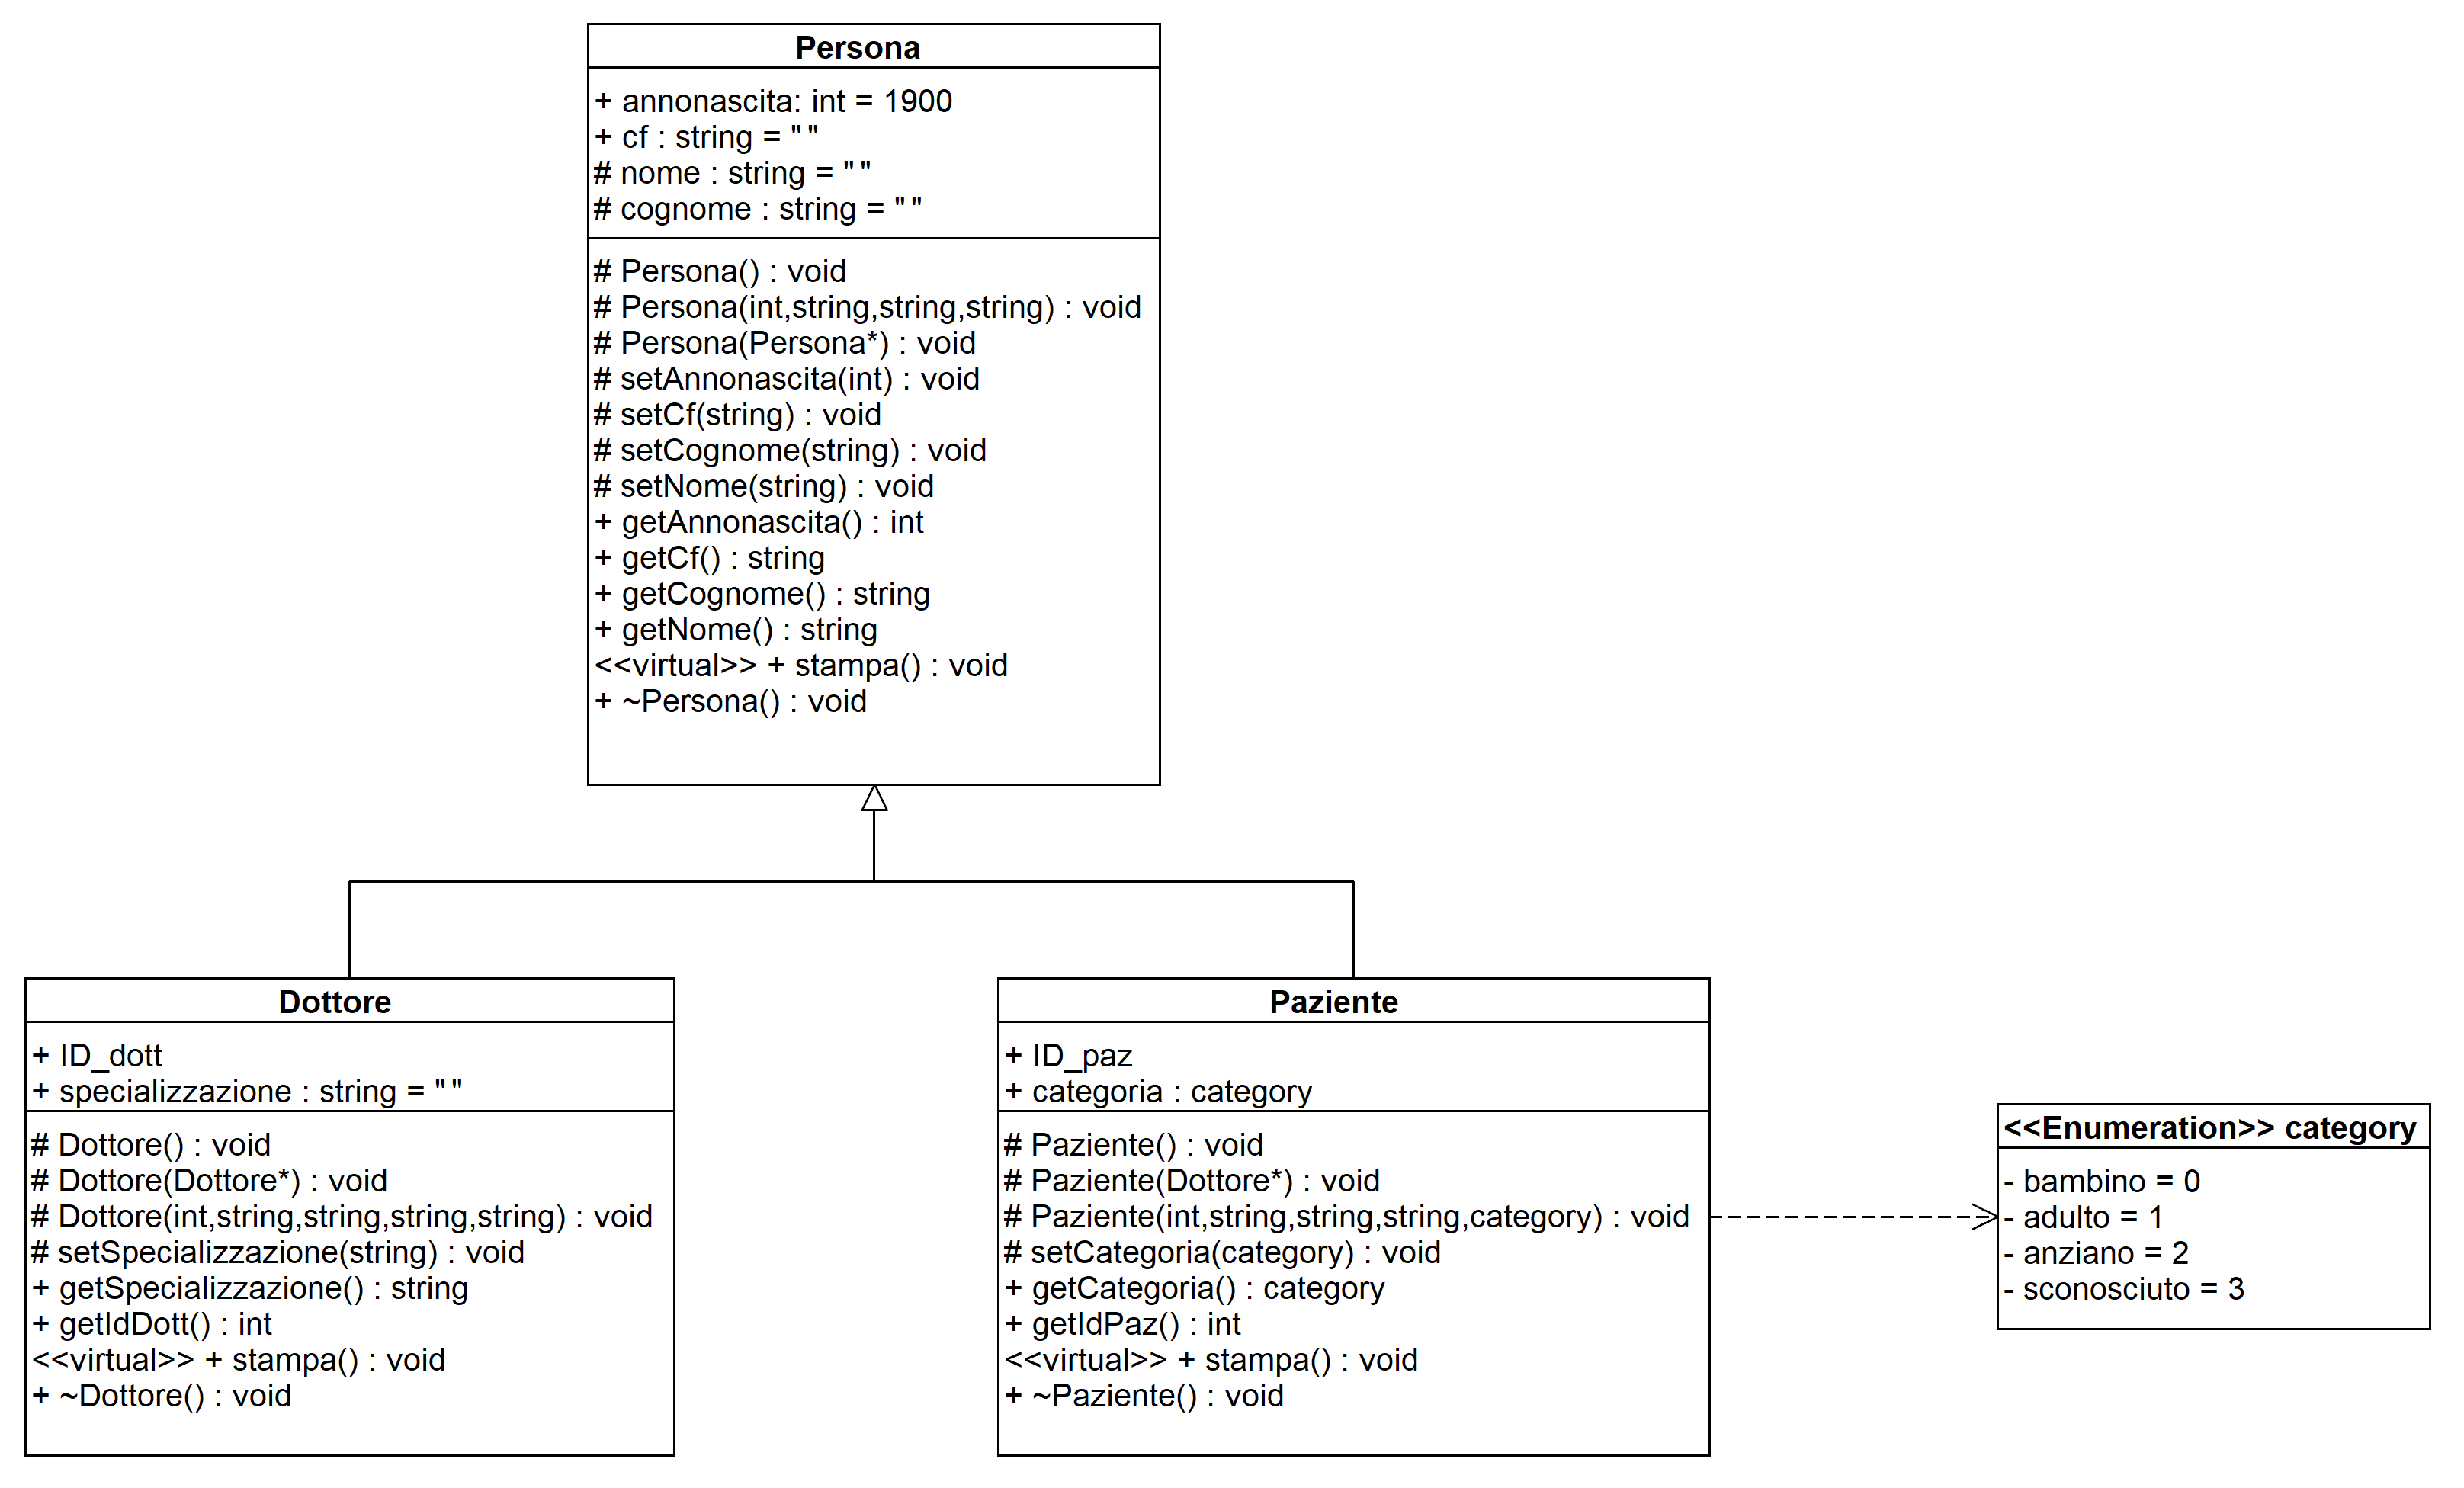
\includegraphics[width=\columnwidth]{diagrammiClassi/gerarchiaPersone}
 \caption{Diagramma delle classi - Gerarchia utenti.}
\end{figure}
\\
\begin{figure}[h]
 \centering
 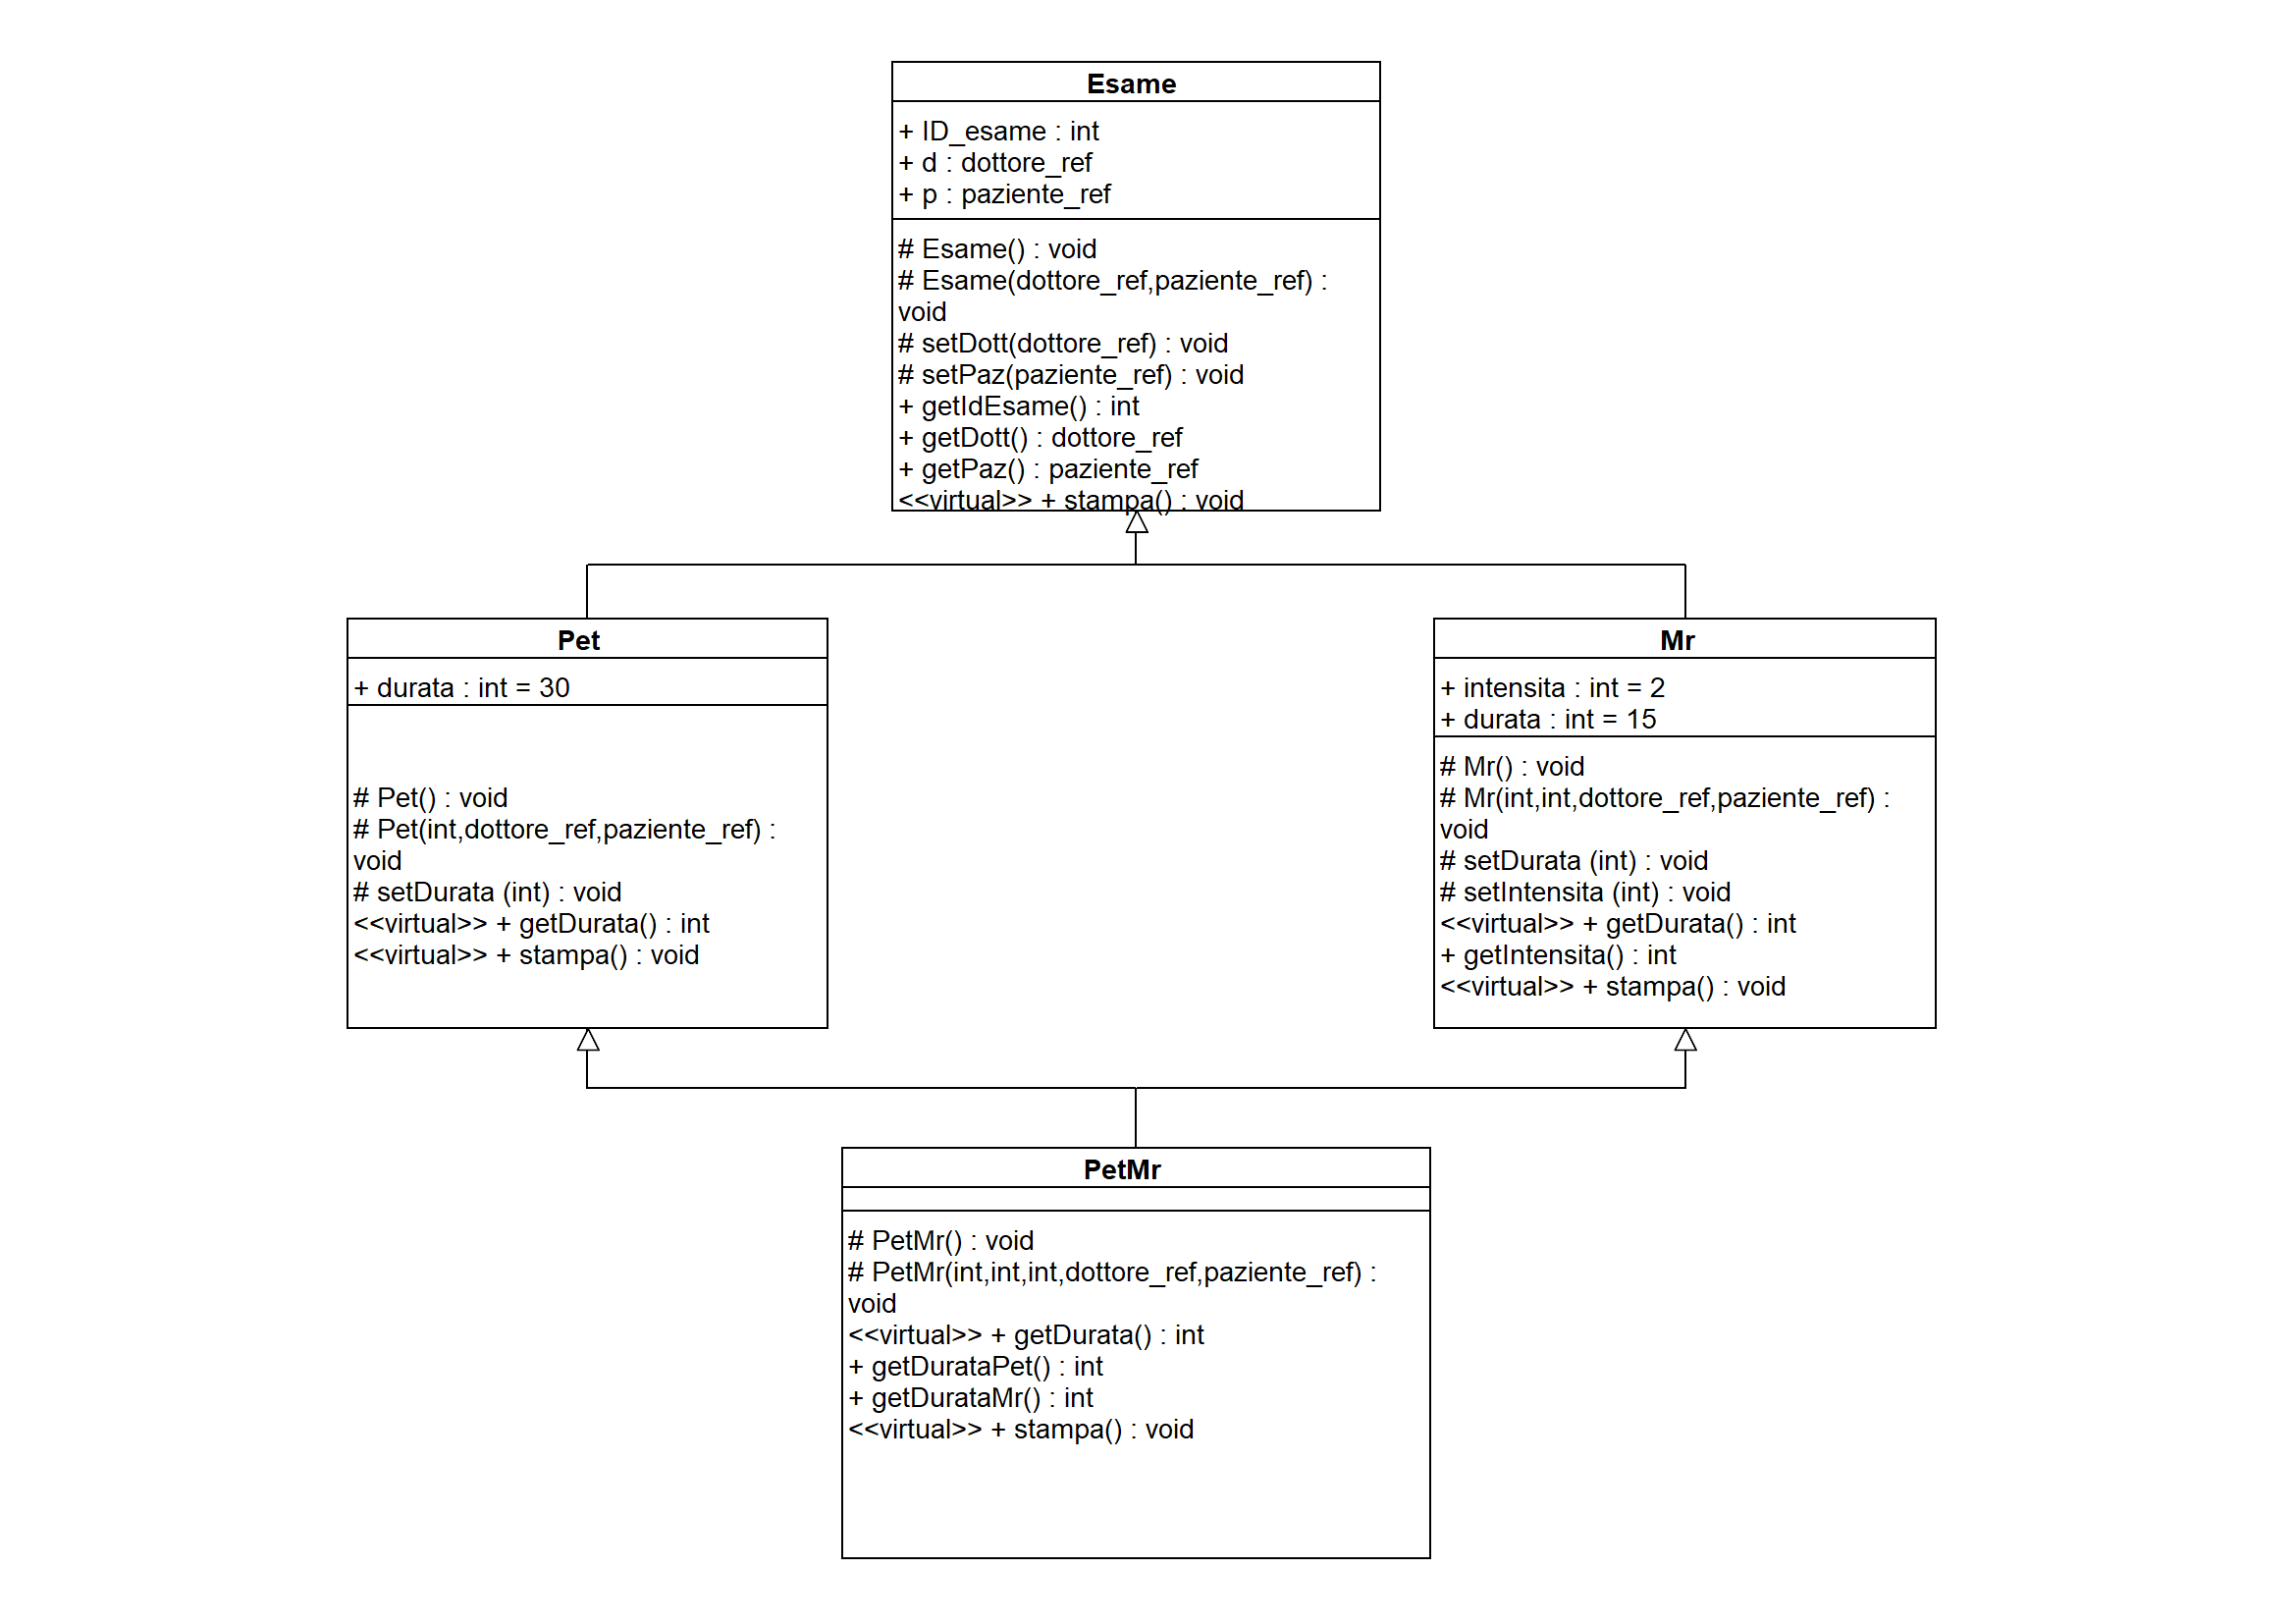
\includegraphics[width=\columnwidth]{diagrammiClassi/gerarchiaEsami}
 \caption{Diagramma delle classi - Gerarchia esami.}
\end{figure}
\\
\begin{figure}[h]
 \centering
 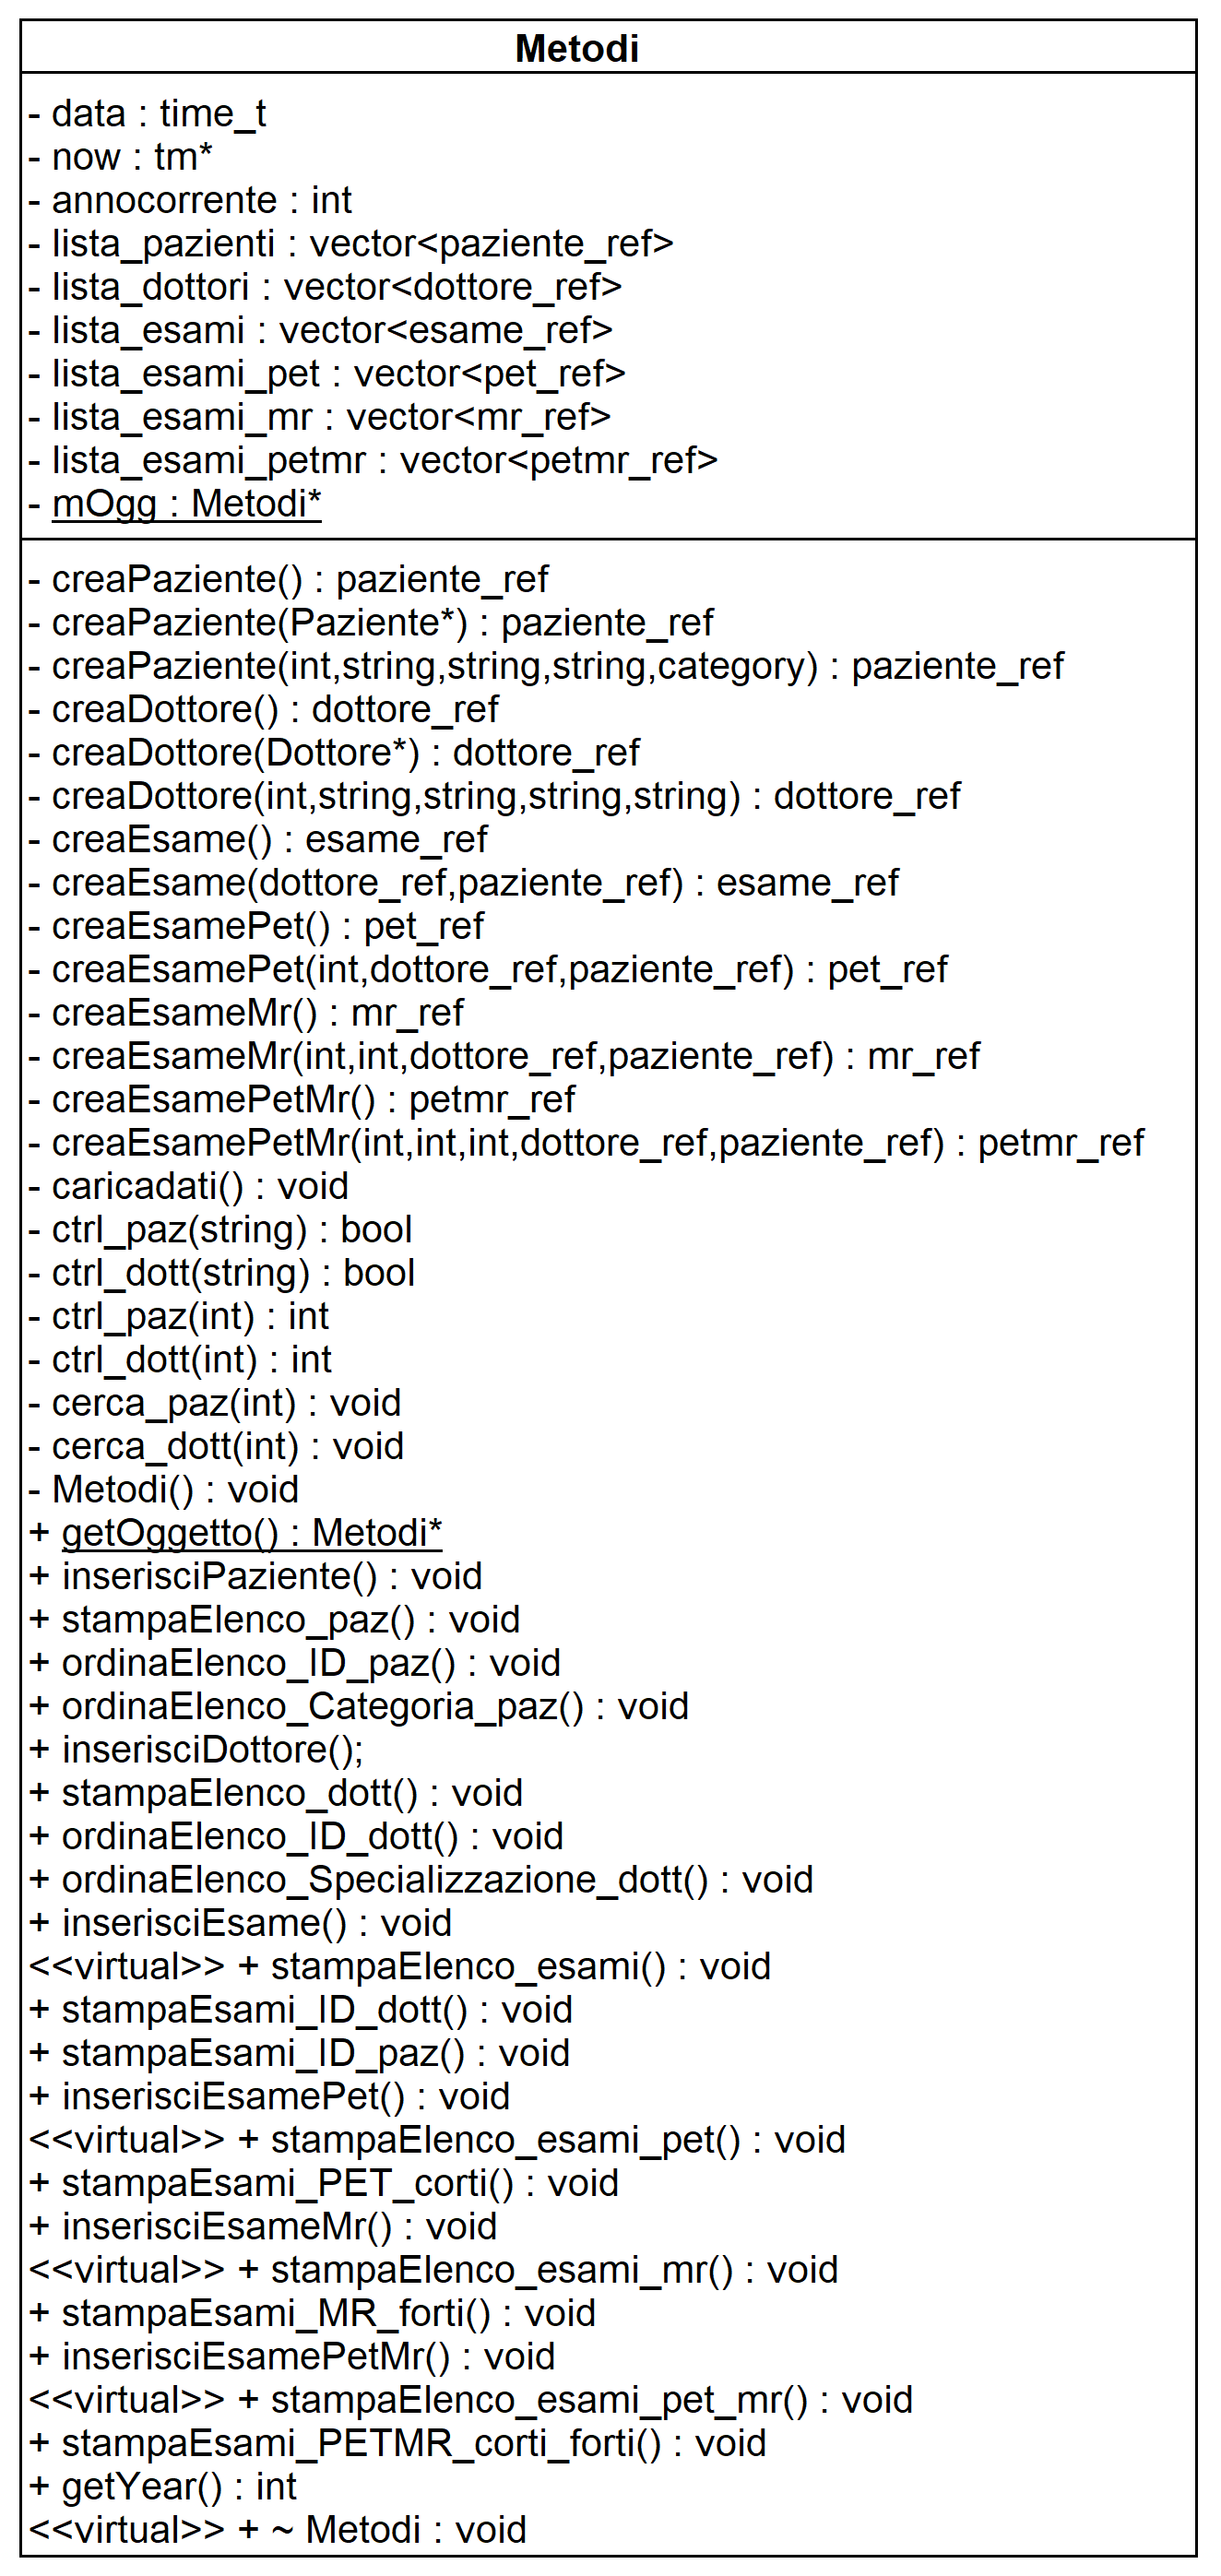
\includegraphics[height=0.9\textheight]{diagrammiClassi/metodi}
 \caption{Diagramma delle classi - Metodi resi disponibili nel programma principale.}
\end{figure}




%----------------------------------------------------------------------------------------

\end{document}
